\section{PCIe and InfiniBand}
\label{sec:pcie}

This section discusses relevant details of PCI Express and InfiniBand, and
discusses what PCIe events are measured by Intel's PCIe counters on different
CPU generations.

\subsection{PCI Express}
PCIe is a serial point-to-point interconnect which is commonly used to connect
peripheral devices to a CPU. The bandwidth of a PCIe link is determined by two
factors: the link width and the PCIe generation. The link width speficies the
number of parallel lanes in the interconnect---the bandwidth of the link is
simply the per-lane bandwidth multiplied by the number of lanes. The PCIe
generation can be any number between 1 and 3, with PCIe 3.0 being the newest
generation at the time of writing. The transfer rate of a PCIe lane has
increased with each PCIe generation; Table~\ref{table:pcie} shows the transfer
rate of different PCIe generations and the bandwidth of a single lane of this
generation. As diffenent PCIe generations use different physical layer encodings
(8b/10b for PCIe 1.0 and 2.0, 128b/130b for PCIe 3.0), the relation between the
transfer rate and useful bandwidth of a PCIe lane depends on the generation. 

\begin{table}
\begin{center}
    \begin{tabular}{p{2.5cm} p{1.5cm} p{2.5cm}}
	\textbf{Generation} & \textbf{Bitrate} & \textbf{Lane bandwidth}\\
    \hline
	PCIe 1.0 & 2.5 GT/s & 250 MB/s \\
	PCIe 2.0 & 5 GT/s & 500 MB/s \\
	PCIe 3.0 & 8 GT/s & 984.6 MB/s \\
    \end{tabular}
\caption{Transfer rate and per-lane bandwidth of different PCIe generations}
\label{table:pcie}
\end{center}
\end{table}

\subsection{PCIe protocol}
PCIe is a layered protocol and consists of a physical layer, a link layer,
and a transport layer. The link layer uses credit-based flow control and
acknowledgments to provide reliable delivery to the transport layer.
Figure~\ref{fig:pcie-tlp} shows the structure of a PCIe 3.0 transaction layer
packet (PCIe TLP). In addition to the data payload, the packet includes physical
layer framing, a link layer sequence number (for reliability), a transport layer
header, and checksum at both the transport and link layer.

For the purposes of this paper, we assume that there are two types of PCIe
operations: memory read and memory write. The type of operation and the memory
address (in the peer's virtual memory) to read or write from is specified
in the transaction layer header. Therefore,  the transaction layer
header can be either 12 or 16 bytes depending on whether 32-bit or 64-bit
addressing is used.  As almost all modern servers use 64-bit addressing, we
assume that the size of the transaction layer header is 16 bytes.

From Figure~\ref{fig:pcie-tlp}, it is clear that the minimum TLP overhead of
a PCIe packet is 30 bytes. Understanding this is crucial to designing better
RDMA-based communication protocols, as we will show in Section~\ref{sec:measurements}.

\begin{figure}
	\centering
	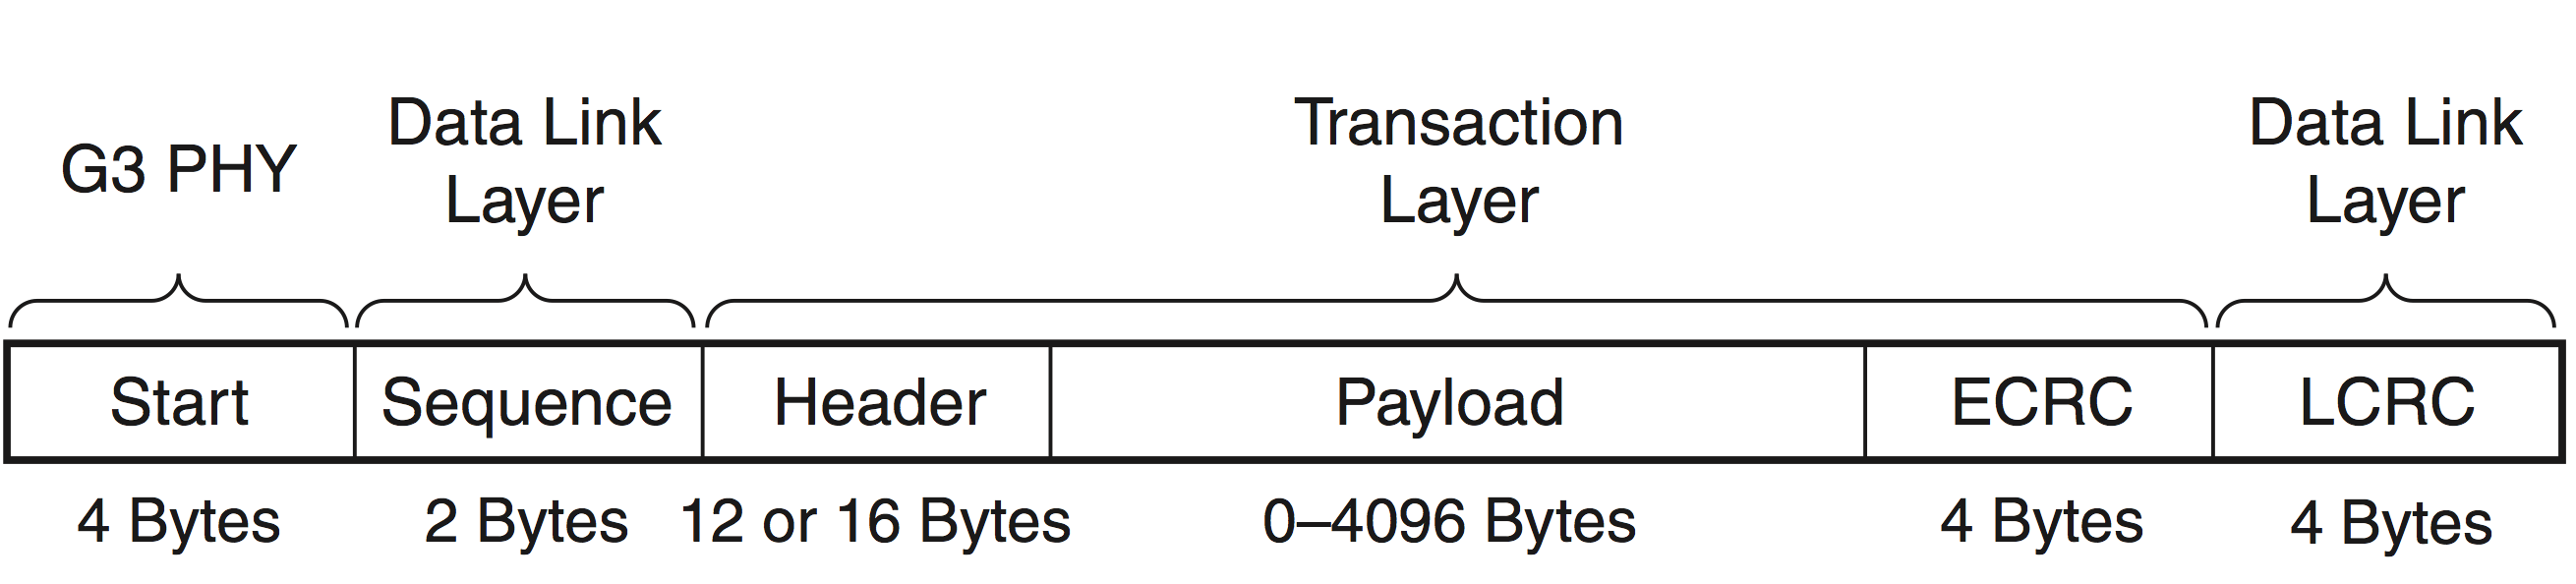
\includegraphics[width=.48\textwidth]{figures/pcie-tlp.png}
	\caption{\textbf{Structure of a PCIe TLP. The diagram was copied from~\cite{www-xilinx-pcie}}}
	\label{fig:pcie-tlp}
\end{figure}
